\chapter{Simplified Parametrisation of the Spiral}
\section{Rationale for the New Parametrisation}
The constants \(\frac{6}{\pi\sqrt{3}}\) and \(\frac{\pi}{\sqrt{3}}\) arise
directly from the asymptotic structure of the arc length of the Archimedean spiral
\(r(\theta)=a\theta\). The exact arc length function reads


\[
L(\theta)=\frac{a}{2}\bigl[\theta\sqrt{\theta^{2}+1}+\operatorname{arcsinh}(\theta)\bigr].
\]


For large \(\theta\), the term \(\theta\sqrt{\theta^{2}+1}\) dominates, so that


\[
L(\theta)\sim \frac{a}{2}\theta^{2}.
\]


With \(a=\frac{6}{\pi^{2}}\), the asymptotic relation


\[
L(\theta)\sim \frac{3}{\pi^{2}}\theta^{2}
\]


follows.

If a parameter \(p\) representing the arc length is introduced, then
the inversion of \(p=L(\theta)\) yields


\[
\theta(p)\approx \sqrt{\frac{2p}{a}}
= \frac{\pi}{\sqrt{3}}\sqrt{p}.
\]


The constant \(\sqrt{3}\) thus arises directly from the quadratic
growth order of the arc length and represents the scaling factor that ensures
the asymptotic identification of the parameter with the arc length.

Since \(r=a\theta\), it follows for the radius that


\[
r(p)=a\,\theta(p)
= \frac{6}{\pi^{2}}\cdot\frac{\pi}{\sqrt{3}}\sqrt{p}
= \frac{6}{\pi\sqrt{3}}\sqrt{p}.
\]



The constant \(\sqrt{3}\) thus possesses an intrinsic geometric meaning:
it characterises the natural scaling required to reparametrise the
spiral so that the new parameter \(p\) generates equidistant
arc lengths. Remarkably, the same constant also appears in the
analysis of the quadratic function


\[
f(x)=\frac{1}{6}(2x^{2}+3x+1)
\]


as the horizontal stretching factor \(1/\sqrt{a}=\sqrt{3}\). Both curves
thus exhibit an identical scaling constant arising from their respective
arc length structures.


\begin{tcolorbox}[
  title={Why a new parametrisation is necessary},
  colback=gray!5,
  colframe=gray!50!black,
  enhanced,
  breakable
]
The standard parametrisation of the Archimedean spiral via the angle \(\theta\) describes the curve geometrically correctly but does not generate arc lengths that correspond to the arithmetic structure of the sequence \(k(n)\). For the present application, a parameter is needed whose increment corresponds directly to the arc length measured along the spiral. By introducing the parameter \(p\), which traverses the values of \(k(n)\), an equidistant arc length scale is created. The spiral remains geometrically unchanged but acquires a parametrisation that precisely reflects the arithmetic structure of the sequence.
\end{tcolorbox}


\begin{figure}[htbp]
  \centering
  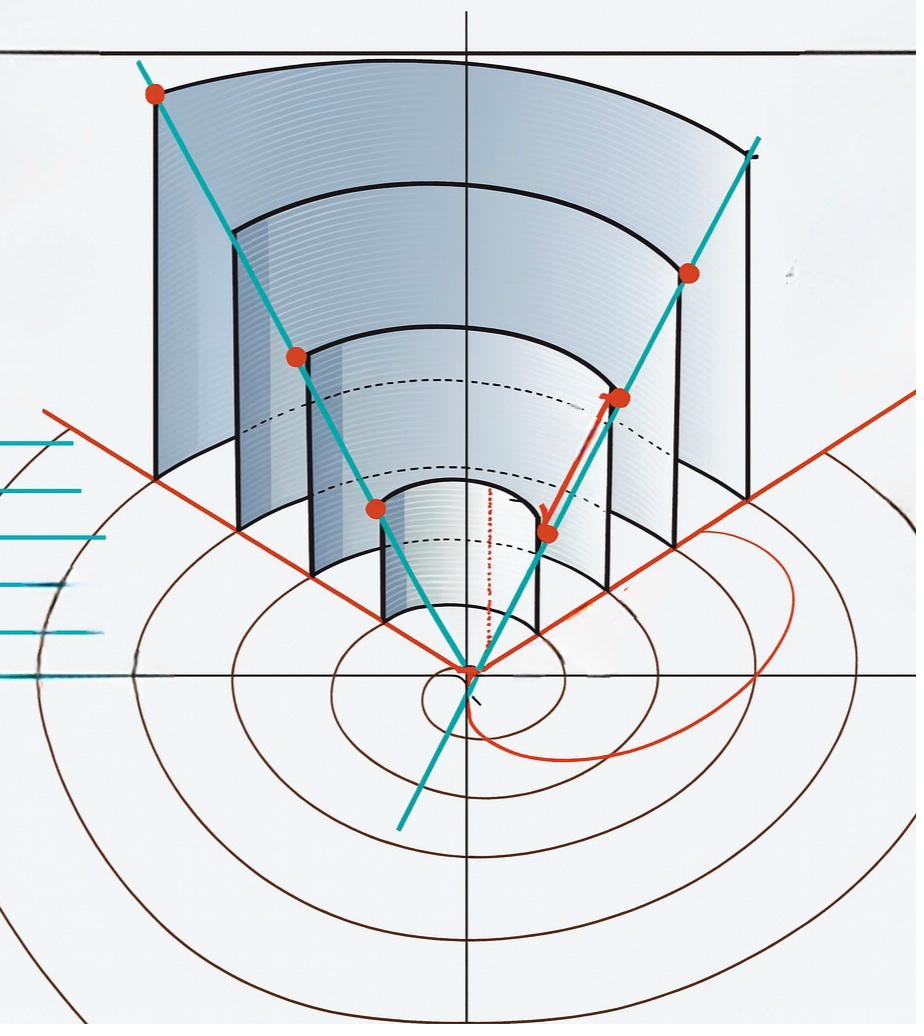
\includegraphics[width=0.78\textwidth]{bilder/spirale_3d_uebergang}
  \caption{Transition from the two-dimensional Archimedean spiral (below)
    to the three-dimensional cylindrical structure (above). The cyan rays
    mark the radius vector $r(\theta)$ at the integer points of the
    sequence; the orange lines visualise the corresponding tangential directions.
    The concentrically arranged circular arcs correspond to the discrete
    radius increments $\Delta r = 12/\pi$, which upon unrolling become the vertical
    spacings of the 3D surface.}
  \label{fig:spirale_3d_uebergang}
\end{figure}

\section{Polar Form with Parameter \texorpdfstring{$p$}{p}}

We introduce a new parameter $p$ that corresponds directly to the integer
function values of the sequence $k(n)$.

\begin{satz}[Simplified polar representation]
The spiral can be expressed in the form
\begin{equation}
\boxed{
\begin{aligned}
r(p) &= \frac{6}{\pi} \cdot \sqrt{\frac{p}{3}} \\
     &= \frac{6}{\pi\sqrt{3}} \cdot \sqrt{p}, \\[6pt]
\theta(p) &= \pi \cdot \sqrt{\frac{p}{3}} \\
          &= \frac{\pi}{\sqrt{3}} \cdot \sqrt{p},
\end{aligned}
}
\end{equation}
where $p$ traverses the values of the sequence $k(n)$.
\end{satz}

With numerical values:
\begin{align}
r(p) &= \frac{6}{\pi\sqrt{3}} \cdot \sqrt{p} \approx 1.102657790844 \cdot \sqrt{p}, \\
\theta(p) &= \frac{\pi}{\sqrt{3}} \cdot \sqrt{p} \approx 1.813799364234 \cdot \sqrt{p}.
\end{align}

\begin{anmerkung}
A common source of error is the confusion of the two equivalent representations
of the radius function. We have
\[
  r(p) = \frac{6}{\pi\sqrt{3}}\,\sqrt{p}
       = \frac{6}{\pi}\,\sqrt{\frac{p}{3}}.
\]
The factor $\frac{6}{\pi} \approx 1.9099$ is the coefficient of $\sqrt{p/3}$, \emph{not} 
of $\sqrt{p}$. If it is directly multiplied with $\sqrt{p}$, the resulting 
coordinates are too large by a factor of $\sqrt{3} \approx 1.732$. 
For numerical evaluations, the form 
$r(p) = 1.102657790844 \cdot \sqrt{p}$ is therefore recommended.
\end{anmerkung}

\section{Parametric Representation in Cartesian Coordinates}

\begin{equation}
\begin{aligned}
x(p) &= r(p)\cos(\theta(p))
     = \frac{6}{\pi\sqrt{3}}\sqrt{p}\,
       \cos\!\left(\frac{\pi}{\sqrt{3}}\sqrt{p}\right), \\[6pt]
y(p) &= r(p)\sin(\theta(p))
     = \frac{6}{\pi\sqrt{3}}\sqrt{p}\,
       \sin\!\left(\frac{\pi}{\sqrt{3}}\sqrt{p}\right).
\end{aligned}
\end{equation}

\section{Derivatives}

\begin{satz}[Derivatives of the polar coordinates]
\begin{equation}
\begin{aligned}
\frac{dr}{dp}
  &= \frac{d}{dp}\left[\frac{6}{\pi\sqrt{3}}\sqrt{p}\right]
   = \frac{6}{\pi\sqrt{3}} \cdot \frac{1}{2\sqrt{p}}
   = \frac{\sqrt{3}}{\pi\sqrt{p}}, \\[10pt]
\frac{d\theta}{dp}
  &= \frac{d}{dp}\left[\frac{\pi}{\sqrt{3}}\sqrt{p}\right]
   = \frac{\pi}{\sqrt{3}} \cdot \frac{1}{2\sqrt{p}}
   = \frac{\pi}{2\sqrt{3}\sqrt{p}}.
\end{aligned}
\end{equation}
\end{satz}

Numerically:
\begin{align}
\frac{dr}{dp} &= \frac{\sqrt{3}}{\pi\sqrt{p}} = \frac{0.551328895422}{\sqrt{p}}, \\[4pt]
\frac{d\theta}{dp} &= \frac{\pi}{2\sqrt{3}\sqrt{p}} = \frac{0.906899682117}{\sqrt{p}}.
\end{align}
